\chapter{Diseño del sistema}   \label{cap:capitulo5}

Como este software va a reutilizar gran parte del software de los limitadores \acrshort{LM7} y la \acrshort{LM9}, se ha decidido bautizar al nuevo limitador como \textbf{LM11}, para poder así referirnos a él de forma breve al mismo tiempo que se mantiene la consistencia en la nomenclatura.

Para la etapa de diseño se tiene en cuenta el estudio y las consideraciones tomadas en los capítulos de Ingeniería Inversa y Análisis, mediante las cuales hemos descubierto las necesidades del sistema que se pretende desarrollar, las características del equipo sobre el que se va a instalar nuestro software y el grado de aceptación del software disponible en base a los requisitos del proyecto.

\begin{figure}[h]
    \centering
    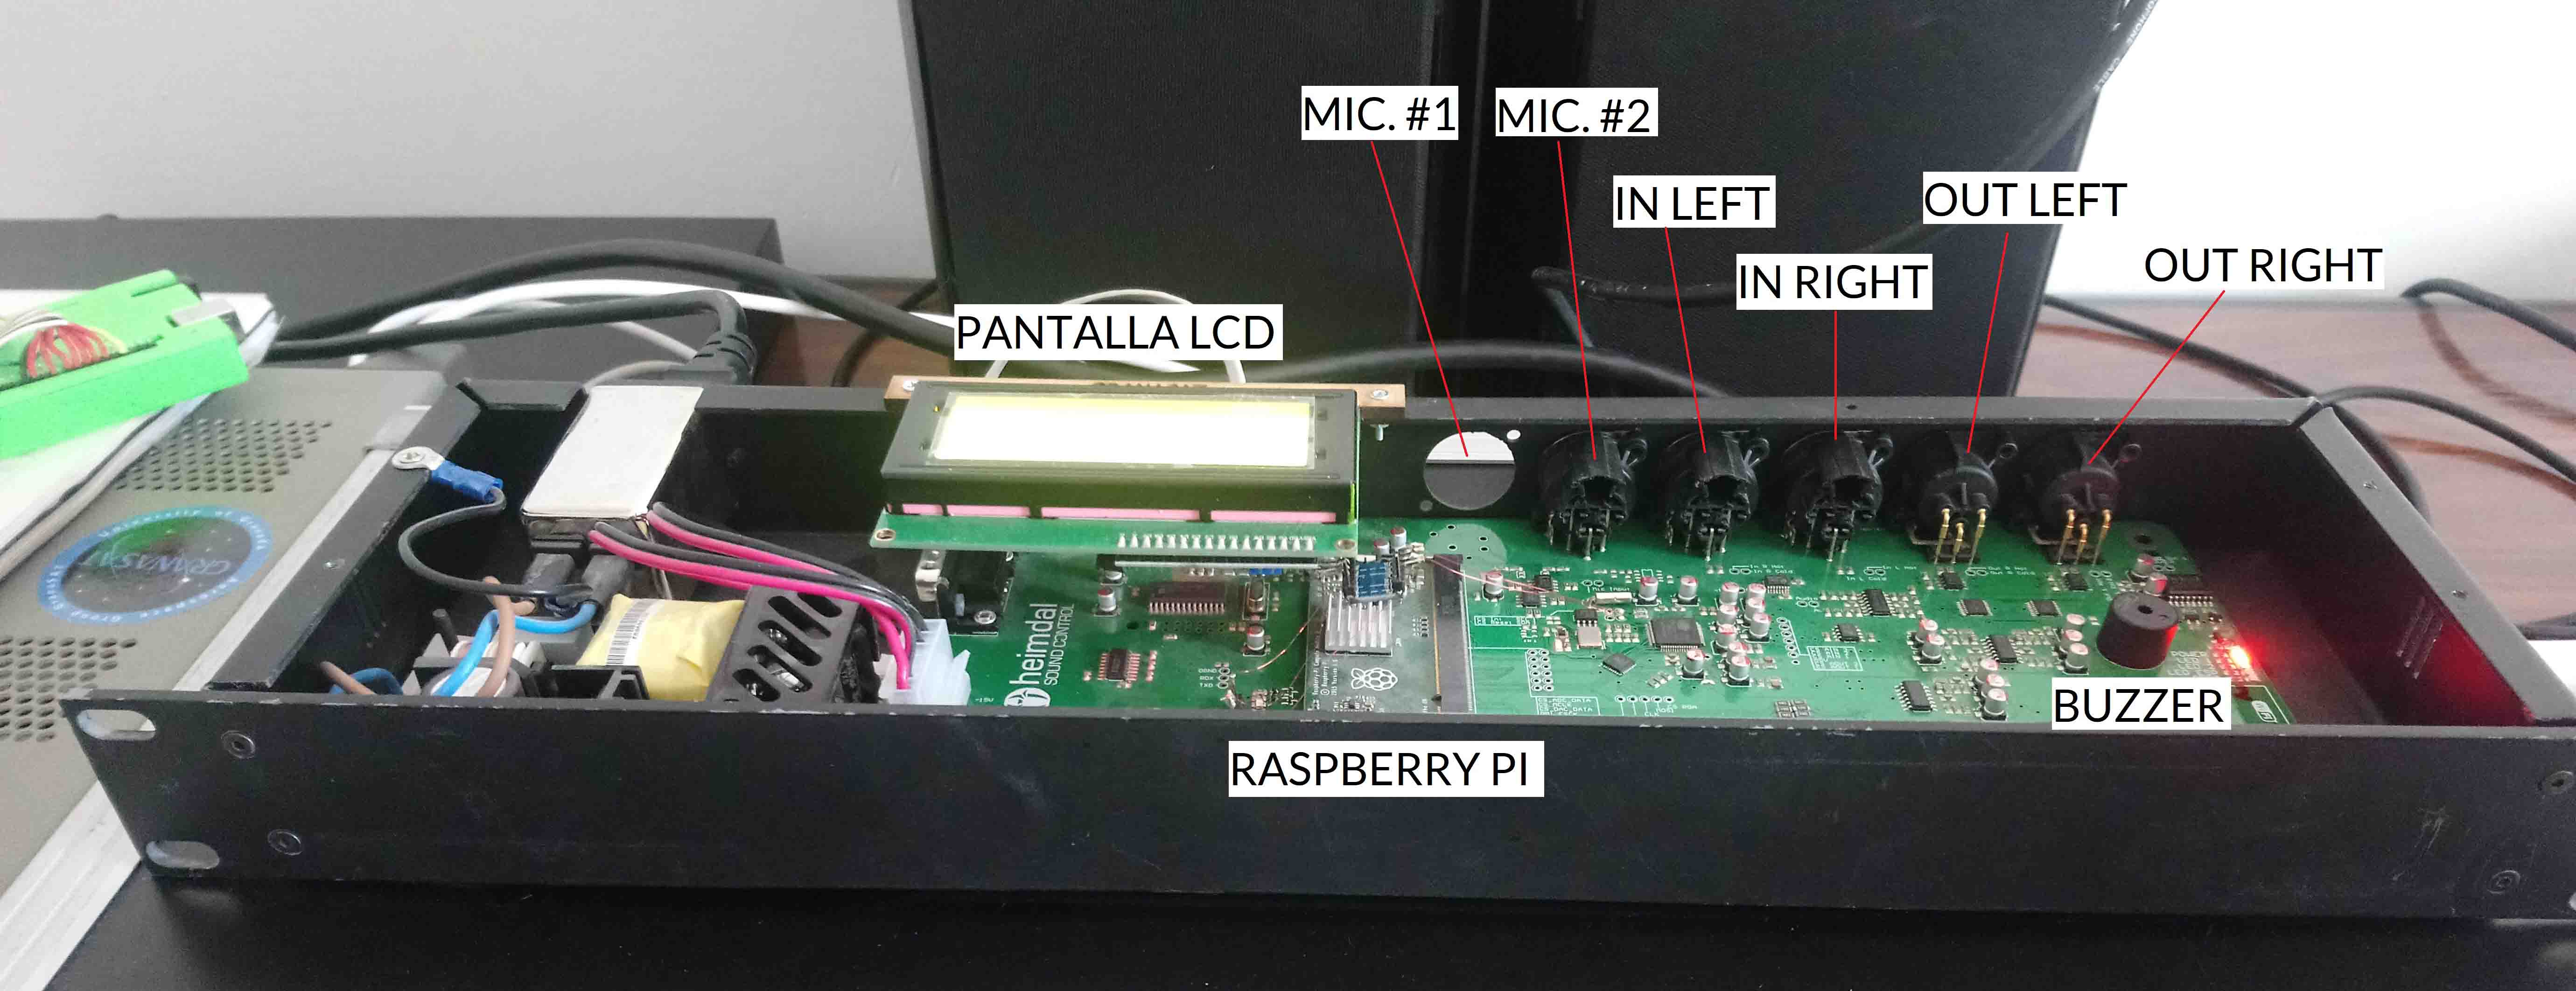
\includegraphics[width=0.9\textwidth]{imagenes/lm7-fotos/lms11-frontal.jpg}
    \caption{Entradas balanceadas \acrshort{XLR} para canales del audio en el \acrshort{LM11}.}
    \label{img:lms11-xlr}
\end{figure}

En la imagen \ref{img:lms11-xlr} podemos ver una imagen del limitador y algunos de sus componentes. Se puede observar con facilidad las importantes diferencias en comparación con el limitador que se ha venido estudiando, el cuál podemos ver en la imagen \ref{img:lms7_open}. Las diferencias son notables, ya que nos encontramos ante un hardware más moderno, compacto y más elaborado, diseñado exclusivamente para éste propósito, mientra que el \acrshort{LM7} utilizaba una placa base de ordenador industrial conectada mediante cables soldados a una pequeña \acrshort{PCB} de fabricación casi casera. El prototipo es bastante más pequeño que el \acrshort{LM7}.

A nivel de sistema, podemos visualizar el nuevo limitador mediante el diagrama \ref{fig:lms11-circuit}. En este diagrama podemos observar que los elementos principales a nivel de hardware son tan solo tres: el módulo de computación (Raspberry Pi), el \acrshort{PGA} y el conmutador. \\
Tanto la música como el audio llegan al software de limitación instalado en la Raspberry mediante \textbf{la tarjeta de sonido} (no representada en el diagrama por simplicidad). El software analiza el audio y decide si debe actuar sobre los niveles de ruido, en cuyo caso \textbf{actúa mediante el \acrshort{PGA}}, conectado a la Raspberry a través de \acrshort{SPI}. El \acrshort{PGA} recibe a su vez el audio de entrada, pero sólo el de la música, y actúa sobre la señal \textbf{aplicando una ganancia}, que puede ser positiva o negativa. Finalmente el audio sale del limitador hacia los amplificadores y/o altavoces \textbf{pasando por el conmutador}, siempre y cuando éste lo permita.

El conmutador proporciona un \textbf{camino único a la salida} de audio del limitador, y solo puede proporcionar este camino a la \acrshort{PGA} o a la Raspberry, pero no a ambos a la vez (de la misma forma que se vio en el LM8 \ref{img:lm7-rele}). Normalmente se encontrará en la posición que se ve en el diagrama, de forma que dé salida al audio procesado por el \acrshort{PGA}, pero en aquellos momentos en los que se requiera \textbf{emitir ruido rosa} para calibrar el sistema o verificar su calibración, se deberá dar salida al audio proveniente de la Raspberry, esto es, el audio que se reproduzca dentro del sistema operativo.

\begin{figure}[h]
    \centering
    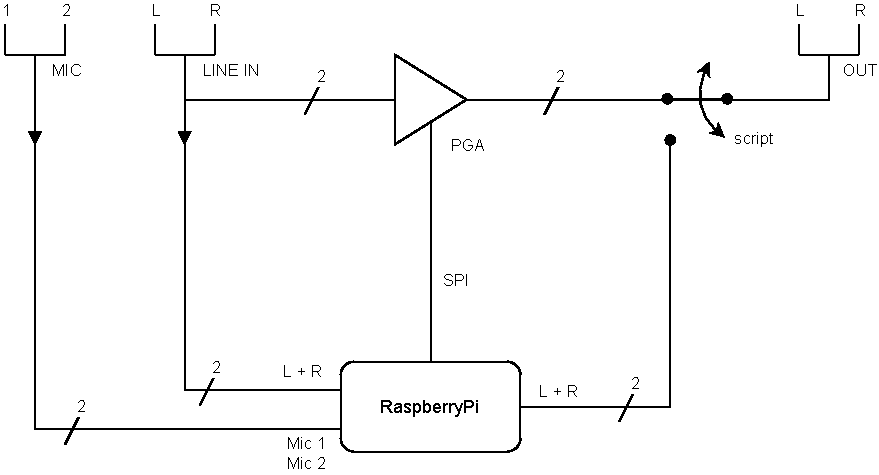
\includegraphics[width=0.9\textwidth]{figuras/lms11-esquema-hardware.pdf}
    \caption{Esquema hardware del limitador \acrshort{LM11}.}
    \label{fig:lms11-circuit}
\end{figure}

Toda la información y conocimiento extraídos del proceso de ingeniería inversa se puede resumir en el esquema de la figura \ref{fig:lms11-software}. Principalmente, se requieren los tres elementos que se ven en el diagrama: un analizador de audio que procese las entradas de audio y genere un modelo con el que poder trabajar; un calibrador; y un limitador, que tome las decisiones oportunas en base al modelo generado, la calibración y la configuración (la normativa).

\begin{figure}[h]
    \centering
    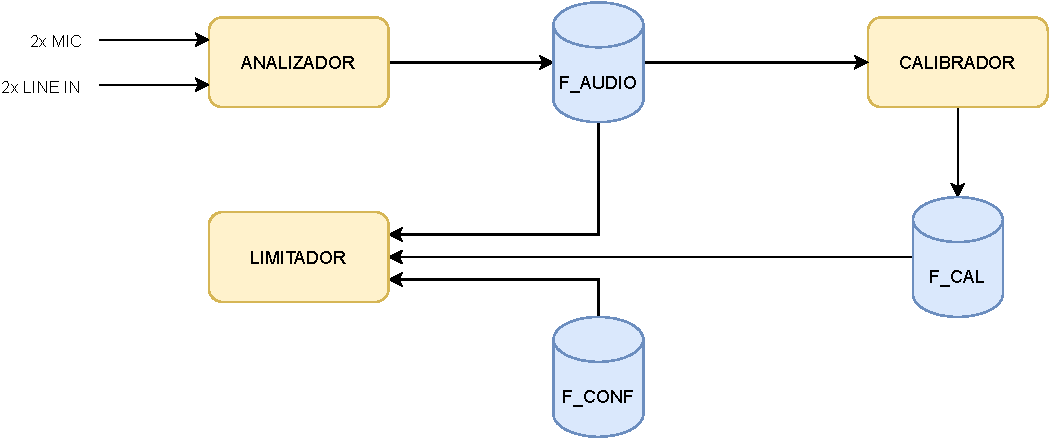
\includegraphics[width=0.9\textwidth]{figuras/lms11-esquema-software.pdf}
    \caption{Esquema software del limitador \acrshort{LM11}.}
    \label{fig:lms11-software}
\end{figure}


Los limitadores estudiados dependían de una aplicación web para su configuración y la consulta de sus datos. Como esta aplicación no se va a importar, debemos buscar otra forma de realizar estas tareas. Como interfaz de comunicación con el exterior del limitador, se propone una \glsname{API-REST} que proporcione una serie de endpoints mediante los cuales se pueda consultar los datos de limitador y configurarlo. El sistema propuesto se traduce en el diagrama \ref{fig:lms11-overview}.

\begin{figure}[h]
    \centering
    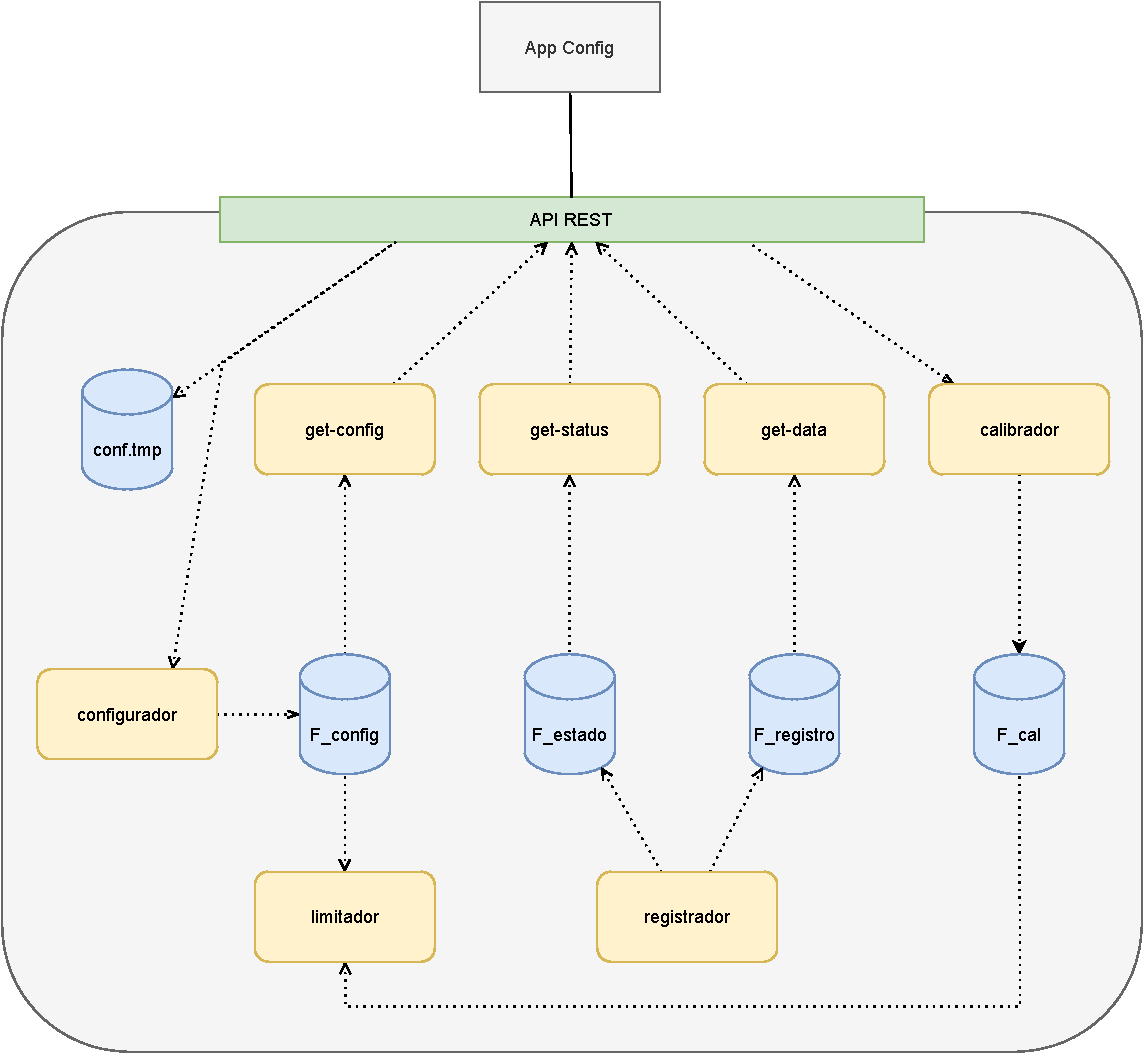
\includegraphics[width=0.9\textwidth]{figuras/lms11-overview.pdf}
    \caption{Esquema parcial del sistema propuesto.}
    \label{fig:lms11-overview}
\end{figure}

\clearpage
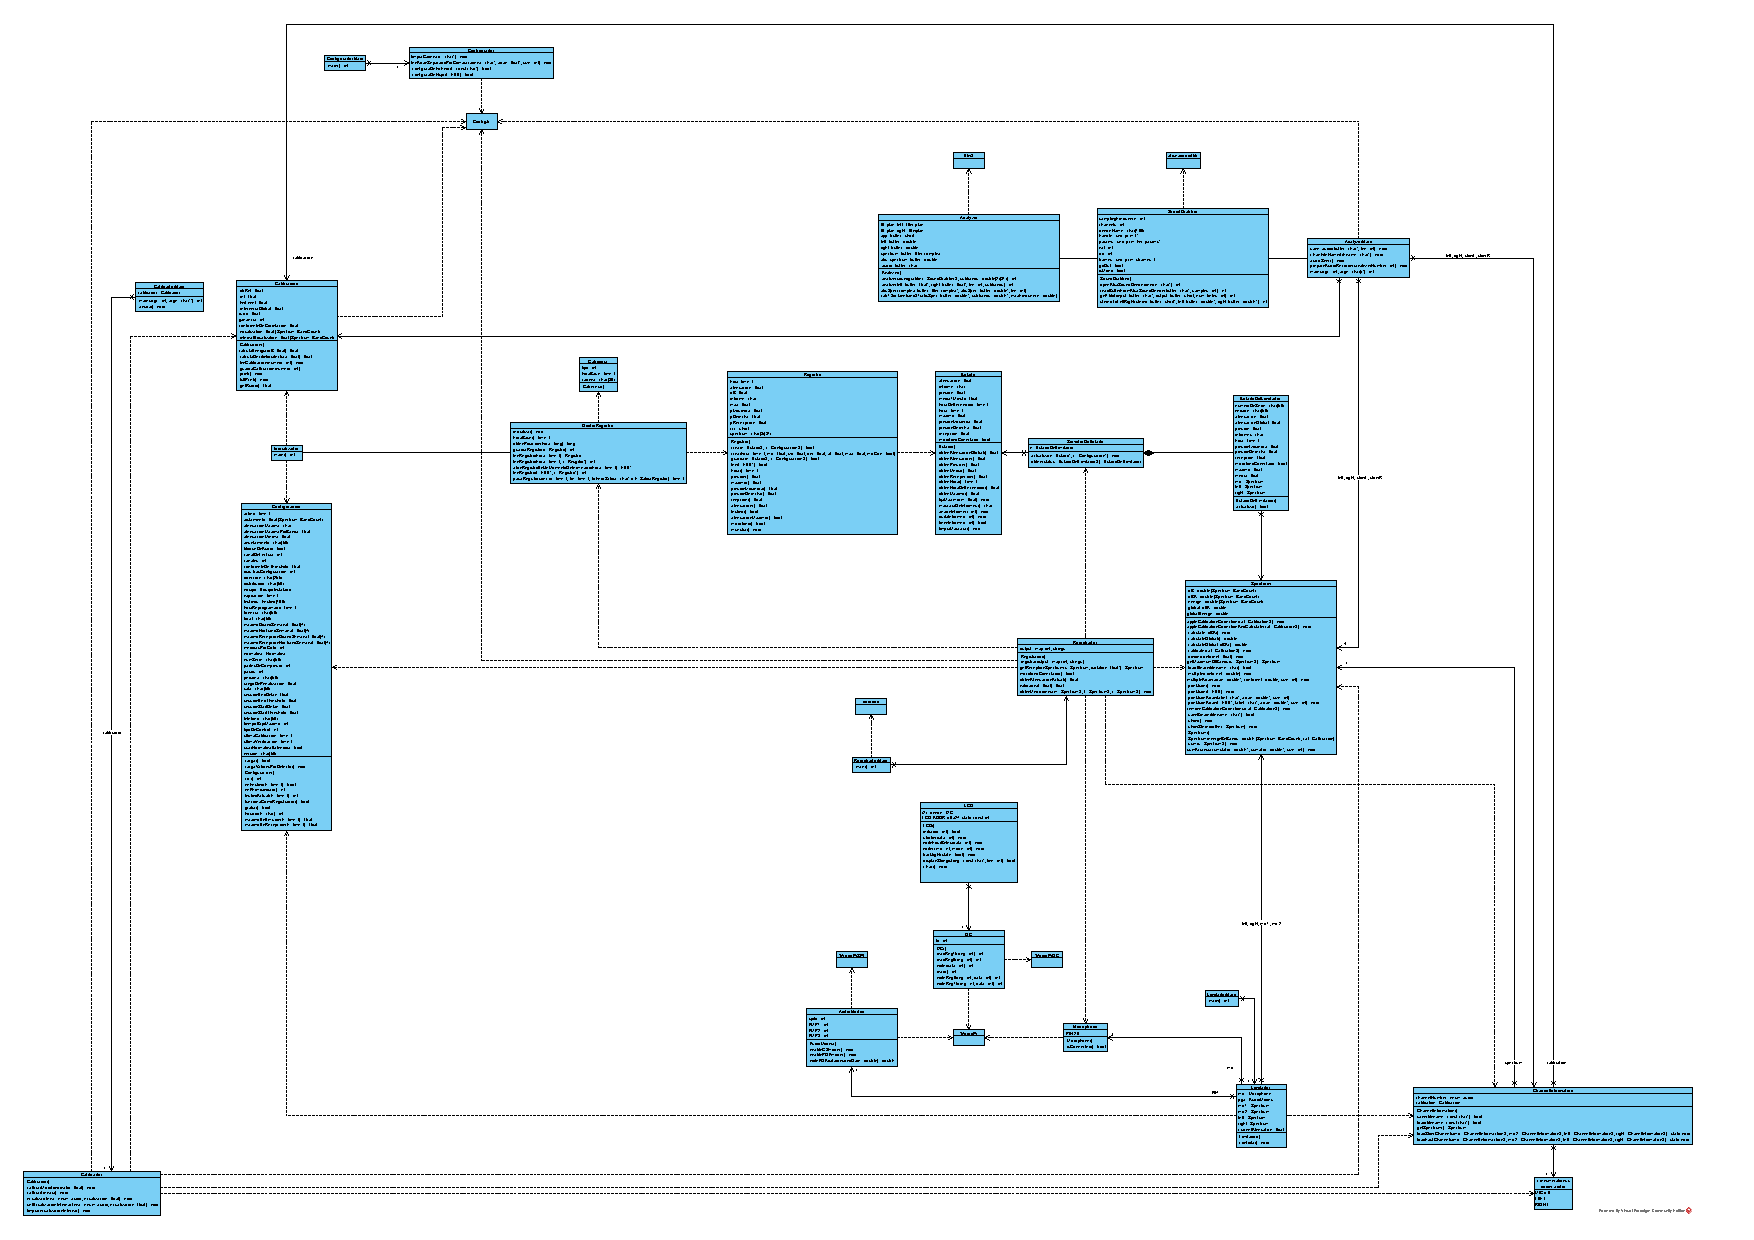
\includepdf[landscape=true]{figuras/lms11-class-diagram.pdf}

\section{Arranque}

\begin{flushright}
\textbf{systemd}
\end{flushright}

Al arrancar el sistema se debe lanzar el software y todos los programas que lo componen. Para ello se propone el uso de un script de arranque definido como un servicio de \glsname{systemd} \cite{systemd}, y por lo tanto, siguiendo la estructura que este gestor exige.

La idea es es definir un servicio que lance el script de arranque contenido en el directorio del proyecto, y este a su vez levante todos los programas necesarios. Distinguimos entonces entre script de arranque principal (\texttt{systemd}) y script de arranque secundario (Bash), De esta forma, cuando se reinicie el servicio, todos los programas del limitador se reiniciarán en bloque. Cada uno de los programas a levantar podrían perfectamente tener su propio servicio, pero por el momento no se va invertir tiempo en eso y se propone como trabajo futuro.

Uno de los procesos que deben levantarse al iniciar el sistema es la aplicación \textit{\textbf{Discovery}} o de descubrimiento, de forma que el limitador puede ser detectado por la aplicación de configuración dentro de la red local, por lo tanto existe una dependencia con el servicio de red, \texttt{networkd}.\\

\begin{lstlisting}[language=sh, caption={Ejemplo de servicio de arranque para el \acrshort{LM11}}, label={lst:lms11-boot}]
[Unit]
Description=GranaSAT SoundLimiter bootup service
After=network.target
StartLimitIntervalSec=0
[Service]
Type=simple
Restart=always
RestartSec=1
User=root
ExecStart=/root/SoundLimiter/scripts/run.sh

[Install]
WantedBy=multi-user.target
\end{lstlisting}

\section{Instalación}

\begin{flushright}
\textbf{Script Bash}
\end{flushright}

El software debe ser instalado en el equipo. Por petición del cliente, los ficheros relativos al nuevo software de limitación deben estar centralizados en un sólo directorio, a diferencia de en el \acrshort{LM7} y \acrshort{LM9} que se encontraban dispersos por el sistema de archivos del sistema (\texttt{/bin}, \texttt{/var}, \texttt{/tmp}, \texttt{/shm}...).\\
El software a desarrollar será centralizado en la carpeta \textbf{\texttt{SoundLimiter}}, y dentro de ella habrá subdirectorios para almacenar y organizar las distintas partes del software (véase la figura \ref{fig:lms11-files}). En el sistema propuesto, se centralizará el software en el directorio \texttt{SoundLimiter}.

Para la instalación del software se propone un script Bash que genere realice las siguientes tareas:
\begin{enumerate}
\item Crear los subdirectorios y ficheros utilizados por el software, así como el ajuste de sus permisos.

\item Instalar las librerías necesarias (\acrshort{ALSA}, \acrshort{FFTW}3 y \textit{\textbf{nCurses5}}).

\item Actualizar el \textit{PATH} del sistema, añadiendo las rutas absolutas a los directorios \texttt{bin/} y \texttt{scripts/} de nuestro proyecto. De esta forma se puede lanzar cualquiera de los programas y scripts sin especificar su ruta.

\item Compilar el código mediante el fichero \textit{Makefile}.

\item Inicializar el registro, invocando al programa \texttt{inicializador}.
\end{enumerate}

La instalación solo es necesaria realizar una vez. También es deseable un script que haga justamente lo contrario, desinstalar el software. Este script tan solo debe restaurar el \textit{PATH} del sistema y eliminar la carpeta del proyecto de forma recursiva.

\section{Detección de micrófono}

\begin{flushright}
\textbf{WiringPI - PIN 28}
\end{flushright}

Para la detección del micrófono se recurre a \myMateLuis\ y \myProf, ya que conocen el hardware del limitador ampliamente mejor que yo. \myMateLuis proporciona un programa de prueba en el que se consulta el estado de conexión del micrófono. Este programa utiliza la librería \glsname{WiringPi}, instalada por defecto en todas las Raspberry Pi.

El código se reduce a llamar a una función de \glsname{WiringPi}, consultando el estado del PIN 28. Si la función devuelve 0, entonces el micrófono está conectado, en otro caso, desconectado. \cite{wiringpi}

\section{Procesamiento de audio}

\subsection{Conexión a tarjetas de sonido}

\begin{flushright}
\textbf{Analizador del LM9 | asound.conf}
\end{flushright}

El procesamiento de audio es en esencia el mismo que en el \acrshort{LM9}, aunque como se ha comentado anteriormente, en este caso tenemos una sola tarjeta de sonido que recibe todos los canales de entrada, en lugar recibir el audio del micrófono y de la música por sendas tarjetas de sonido.

De cara a permitir la reutilización de este módulo en nuestro proyecto, debemos encontrar una forma de que se puedan lanzar dos instancias del mismo programa para que lean de canales distintos de la tarjeta de sonido. Por suerte para nosotros, el prototipo viene semi-configurado para ello mediante el fichero de configuración global de \acrshort{ALSA} \textbf{\texttt{asound.conf}}, localizado en el directorio \texttt{/etc}. Tras un extenso estudio de la arquitectura de \acrshort{ALSA} y con configuraciones, se identifica que la configuración existente mapea los canales 0 y 7 (\textbf{canal de entrada izquierdo} y \textbf{canal de entrada derecho} respectivamente) a un \acrshort{PCM} \cite{alsa-pcm} con el nombre \commillas{airplay}. Pasando este nombre el analizador podemos conectarnos y a los canales de entrada por los que se recibe la música.

A cada uno de los canales de la tarjeta de sonido del prototipo le corresponde un número positivo a modo de identificador. En los diagramas técnicos del prototipo, encontramos que los canales vienen dados tal y como se ve en la tabla \ref{tab:lms11-canales}.

\begin{figure}[ht]
    \centering
    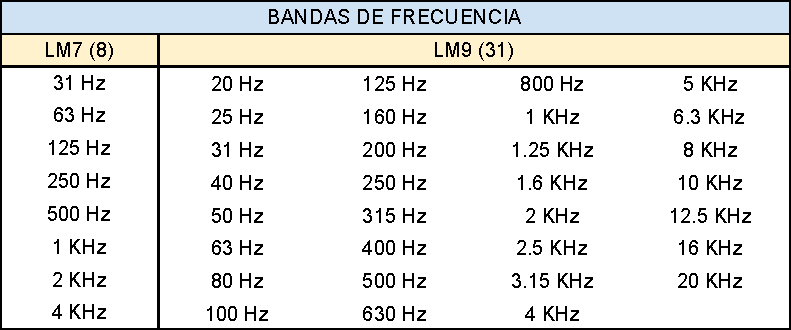
\includegraphics[width=0.8\textwidth]{figuras/lms-frecuencias.pdf}
    \caption{Bandas de frecuencias de los limitadores.}
    \label{fig:lms-freq}
\end{figure}

Con esta información podemos completar la configuración de \acrshort{ALSA} para crear un nuevo \acrshort{PCM} que nos proporcione el audio de los micrófonos. Como el prototipo tiene tan sólo un micrófono instalado de momento, solo se ha generado la configuración para el micrófono \#2 (ver imagen \ref{img:lms11-xlr}). Añadir el primer micrófono al nuevo \acrshort{PCM} resulta trivial, tan sólo hay que añadir la línea \texttt{ttable.0.2 2}, que significa \commillas{mapea al canal 2 de este \acrshort{PCM} el canal 2 del dispositivo 0)}.

Una vez configurado \acrshort{ALSA}, podemos usar los analizadores de audio conectándolos a los \acrshort{PCM} con nombre \commillas{airplay} y \commillas{mic}, en lugar de usar la tarjeta de sonido de forma global (\commillas{hw:0,0}).

\newpage

\begin{lstlisting}[language={conf}, caption={Fichero asound.conf completamente configurado}, label={lst:lms11-asound}]
# Record mixer
pcm.mixin {
  type dsnoop
  ipc_key 1024
  ipc_key_add_uid false
  ipc_perm 0666            # mixing for all users
  slave {
    pcm "hw:0,0"
    channels 8
    period_time 0
    period_size 1024
    buffer_size 8192
    rate 48000
  }
  bindings {
    0 1   # Mic:   map channel 0 on this device to channel 1 on slave device
    1 0   # Left:  map channel 1 on this device to channel 0 on slave device
    2 7   # Right: map channel 2 on this device to channel 7 on slave device
  }
}
# Microphone channel
pcm.mic {
  type plug
  slave.pcm "mixin"  # Mic: map channel 0 on this device to channel 0
  ttable.0.0 1       # on slave device with 100% volume.
}
# Input channels
pcm.input {
  type plug
  slave.pcm "mixin"
  ttable.0.1 1  # Left: map channel 0 on this device to channel 1
                # on slave device with 100% volume.
  ttable.1.2 1  # Right: map channel 1 on this device to channel 2
                # on slave device with 100% volume.
}
# Playback mixer
pcm.mixout {
  type dmix
  ipc_key 2048
  ipc_key_add_uid false
  ipc_perm 0666            # mixing for all users
  slave {
    pcm "hw:0,0"
    channels 8
    period_time 0
    period_size 1024
    buffer_size 8192
    rate 48000
  }
  bindings {
    0 4   # Left:  map channel 1 on this device to channel 4 on slave device
    1 3   # Right: map channel 2 on this device to channel 3 on slave device
  }
}
# Output channels
pcm.airplay {
  type plug
  slave.pcm "mixout"
  ttable.0.0 1
  ttable.1.1 1
}
\end{lstlisting}

\begin{table}[h]
\centering
\begin{tabular}{l|l}
0 & Línea de entrada izquierda \\
7 & Línea de entrada derecha   \\
1 & Micrófono \#1              \\
2 & Micrófono \#2              \\
5 & Línea de salida izquierda  \\
6 & Línea de salida derecha
\end{tabular}
\caption{Canales del limitador de GranaSAT.}
\label{tab:lms11-canales}
\end{table}

\subsection{Interpretación de datos}

\begin{flushright}
\textbf{Analizador del \acrshort{LM9} | Librería \acrshort{FFTW}}
\end{flushright}

Heredado del \acrshort{LM9}, ver \ref{sec:lms9-audio}. No se prevén cambios más allá del refactoring requerido por los problemas descritos en el capítulo \ref{sec:errores}.

\subsection{Almacenamiento de audio}

\begin{flushright}
\textbf{Ficheros \textit{slow} y \textit{fast} | \texttt{SoundLimiter/tmp}}
\end{flushright}

Los ficheros de audio serán los mismos que el \acrshort{LM9}, con la diferencia de que van a ser centralizados y se van a almacenar dentro de la carpeta del proyecto: \texttt{SoundLimiter/var}.

Ver figura \ref{fig:lms9-audio-files}.

\section{Gestión de calibración}

\subsection{Proceso de calibración}

\begin{flushright}
\textbf{Calibrador | \glsname{API-REST}}
\end{flushright}

El proceso de calibración se encuentra como parte de la funcionalidad que ofrece el programa \texttt{localservice} en los limitadores estudiados. Para nuestro sistema, se va a recortar la funcionalidad relativa a la calibración de este programa y se va a llevar a un programa independiente, el Calibrador. Este programa ya existe de hecho en la versión 9 pero no contiene la funcionalidad completa ya que solo puede calibrar las líneas y no el micrófono. Para nuestro software se desea que este programa implemente ambas cosas y se puede tener un programa exclusivamente dedica a calibrar el sistema.

\subsection{Ecualizaciones}

\begin{flushright}
\textbf{Ficheros de calibración | \glsname{API-REST}}
\end{flushright}

Se utilizarán las mismas ecualizaciones vistas en el \acrshort{LM9} (\ref{sec:lms11-eq}), con la diferencia de que ahora se configurarán y consultarán mediante la \glsname{API-REST} del limitador.

\subsection{Emisión de ruido rosa}

\begin{flushright}
\textbf{Scripts | \glsname{API-REST}}
\end{flushright}

Para la emisión del ruido rosa en el nuevo software se va a utilizar el fichero audio del \acrshort{LM7} \texttt{pink.wav}. Para emitir ruido rosa simplemente reproducimos el fichero de audio. Para ello, se van a implementar dos scripts sencillos para lanzar y parar el ruido rosa (\texttt{play-pink.sh} y \texttt{stop-pink.sh}). La reproducción del fichero se realizará mediante \acrshort{ALSA}, con la orden \texttt{\textbf{aplay}}.

Para poder emitir ruido rosa debemos primero conectar la salida de audio de la Raspberry Pi a la salida de audio del equipo (ver diagrama \ref{fig:lms11-circuit}). Para ello se disponen de dos scripts proporcionados por \myMateLuis\ para cambiar la salida del \acrshort{PGA} a la tarjeta de sonido y viceversa. Estos scripts reciben el nombre de \texttt{pgamode.sh} y \texttt{csmode.sh}.

Para poder activar/desactivar el ruido rosa de forma remota, se proveerá de sendos \textit{endpoints} en la \glsname{API-REST} del limitador.

\subsection{Verificación: sesiones}

\begin{flushright}
\textbf{Script del \acrshort{LM7}}
\end{flushright}

Para el control de la sesiones de ruido y la verificación automática de las calibraciones se va a reutilizar el script del \acrshort{LM7}, junto con las dependencias que éste requiere para su funcionamiento.

\subsection{Almacenamiento de calibraciones}

\begin{flushright}
\textbf{Ficheros | \texttt{SoundLimiter/var}}
\end{flushright}

El almacenamiento de las calibraciones será idéntico al visto en el \acrshort{LM7} y \acrshort{LM9}, con la diferencia de que van a ser centralizados en el directorio del proyecto:\\ \texttt{SoundLimiter/var}.

\section{Gestión de la configuración}

\subsection{Proceso de configuración}

\begin{flushright}
\textbf{Configurador | \texttt{conf.tmp} | \glsname{API-REST}}
\end{flushright}

La configuración del nuevo sistema ya no realizará mediante la aplicación web vista en el capítulo \ref{cap:capitulo3_I}. En su lugar, se propone una \glsname{API-REST} para la consulta del estado del limitador y su configuración.

Durante el proceso de ingeniería inversa se averiguó que la configuración a modificar pasaba por un fichero plano antes de ser recuperada y aplicada por el configurador, el cual era parte del programa \texttt{localservice}. El sistema a desarrollar va a utilizar este fichero y a mantener el formato con el fin de poder reutilizar el proceso de configuración lo máximo posible.\\
Por otra parte, como el proceso de calibración se encuentra embebido en un programa que no va a ser de utilidad para nosotros, se va a extraer esta funcionalidad a un nuevo programa independiente, con el fin de no importar más código del estrictamente necesario.

En resumen, el proceso de configuración se compondrá de tres partes bien definidas: la \glsname{API-REST}, el fichero de configuración temporal (en formato de texto plano) y el configurador.\\
La \glsname{API-REST} recibirá la nueva configuración en formato \acrshort{JSON} y llevará estos datos al fichero temporal con un formato que el configurador entiende, para finalmente invocar al programa \texttt{Configurador} para que lee y aplique la nueva configuración. Para más información sobre el fichero temporal y su formato se puede consultar el anexo \ref{append:F_conf.tmp}.

\subsection{Almacenamiento de la configuración}

\begin{flushright}
\textbf{Fichero}
\end{flushright}

El fichero de configuración será el mismo que en la versiones estudiadas pero será centralizado al directorio dedicado al limitador: \texttt{SoundLimiter/var/configuracion}

\begin{figure}[h]
    \centering
    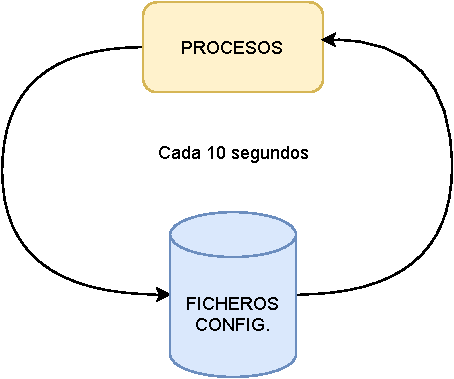
\includegraphics[width=0.45\textwidth]{figuras/lms-conf-reload.pdf}
    \caption{Recarga de ficheros de configuración y calibración.}
    \label{fig:lms-conf-reload}
\end{figure}

\subsection{Consulta de la configuración}

\begin{flushright}
\textbf{Fichero | \texttt{get-config} | \glsname{API-REST}}
\end{flushright}

La lectura de la configuración se realizará mediante el uso del programa \texttt{get-config}, al igual que en el \acrshort{LM7} y el \acrshort{LM9}. La \glsname{API-REST} consultará este programa y devolverá los datos en formato \acrshort{JSON}. Puede verse el anexo \ref{append:getConfig} para más detalles.

\section{Gestión de registros}

\subsection{Proceso de registro}

\begin{flushright}
\textbf{Registrador del \acrshort{LM9}}
\end{flushright}

El proceso de registro va a ser el mismo que el del \acrshort{LM9}, pero para poder reutilizarlo deben arreglase algunos problemas, como los listados en el apartado \ref{sec:errores}. Este programa se compone esencialmente de un \texttt{main()} y varias funciones y variables globales. La idea es llevar esto a una clase y separar el bucle principal del algoritmo de registro. Además, las inclusiones directas de ficheros fuente deben eliminarse, así como todas las inclusiones de ficheros que no sean estrictamente necesarias.

\subsection{Almacenamiento de registros}

\begin{flushright}
\textbf{Fichero | \texttt{SoundLimiter/var}}
\end{flushright}

El almacenamiento de los registros se realiza de forma análoga a como se ha visto en el \acrshort{LM7} y en el \acrshort{LM9}, pero centralizando el fichero al directorio del proyecto: \texttt{SoundLimiter/var/registro.slr}.\\
Además, se va a cambiar el tipo de fichero a un fichero binario común, en lugar de utilizar un fichero especial de bloques como se vio en \ref{img:registro.slr}.

\subsection{Consulta de registros}

\begin{flushright}
\textbf{Fichero | \texttt{get-data} | \glsname{API-REST}}
\end{flushright}

Para la consulta de los registros se reutilizará el programa \texttt{get-data} y se conectará con la \glsname{API-REST}. El usuario proporciona los parámetros requeridos al endpoint de la \glsname{API-REST}, ésta consulta al programa \texttt{get-data} y devuelve los datos en \acrshort{JSON}. El anexo \ref{append:getData} amplia la información sobre este programa.

\section{Proceso de atenuación}

El proceso de atenuación del \acrshort{LM9} parece demasiado complejo en comparación con el del \acrshort{LM7}, y no se comprende del todo su funcionamiento. Por otra parte, tampoco se tiene ninguna certeza de que realmente esa implementación funcione, por lo tanto, se va a romper con la tendencia y en este caso se va a preferir el proceso de atenuación del \acrshort{LM7} \ref{sec:lms7-atenuacion}.

\subsection{Comunicación con el PGA}

La comunicación con el \acrshort{PGA} se va a realizar mediante el uso de la clase \texttt{AudioModes} que puede verse en el diagrama de clases \ref{fig:lms11-clases}. Simplemente se llamará al método \texttt{writePGAdata} pasándole la ganancia deseada como parámetro.